\documentclass[11pt,a4paper]{article}

\usepackage[margin=1in]{geometry}
\usepackage{amsmath,amssymb}
\usepackage{graphicx}
\usepackage{booktabs}
\usepackage{hyperref}
\usepackage{natbib}
\usepackage{microtype}
\usepackage{xcolor}
\usepackage{caption}
\usepackage{subcaption}
\usepackage{multirow}
\usepackage{siunitx}
\usepackage{array}

\hypersetup{
  colorlinks=true,
  linkcolor=blue!70!black,
  citecolor=blue!70!black,
  urlcolor=blue!70!black,
}

\title{\textbf{Pretraining Contamination Does Not Inflate Drug-Target\\
Interaction Benchmarks: A Causal Analysis}}

\author{
  Sam Meyer\\
  Independent Research\\
  \texttt{recons\_01\_frigate@icloud.com}
}

\date{April 2026}

\begin{document}
\maketitle

\begin{abstract}
Drug-target interaction (DTI) prediction benchmarks (Davis, KIBA) are widely used to evaluate
pretrained molecular and protein encoders such as ESM-2 and ChemBERTa.
A standing concern is that these benchmarks may be artificially inflated by \emph{pretraining
contamination}: benchmark compounds or protein sequences appearing in the encoders'
pretraining corpora before the benchmark cutoff date.
We design a causal difference-in-differences (DiD) test to isolate contamination effects.
The \emph{treated} model (ESM-2 + ChemBERTa frozen probe) uses pretrained encoders
subject to corpus overlap; the \emph{control} model (DeepDTA, trained from scratch) provides
a contamination-free baseline.
A clean holdout of 801 post-2021 ChEMBL34 pairs with Tanimoto similarity $<0.4$ to any
training compound serves as the uncontaminated arm.
We additionally ablate pretraining by training an identical MLP on random-weight encoders.
The DiD estimate is strongly \emph{negative} across Davis (DiD$=-0.43$, 95\% CI $[-0.53,
-0.34]$) and KIBA (DiD$=-0.46$, 95\% CI $[-0.55, -0.37]$), with one-sided $p=1.0$ against
the contamination hypothesis.
The random-weight ablation nearly matches ESM-2 on both benchmarks (Davis: $r=0.650$ vs.\ $0.666$;
KIBA: $r=0.786$ vs.\ $0.786$), confirming that pretraining contributes negligible signal
to benchmark performance.
However, \emph{all three models collapse on the holdout}: Pearson $r = 0.017$ (ESM-2),
$-0.375$ (DeepDTA), and $-0.287$ (random).
Davis and KIBA do not measure generalisation to novel chemistry;
this---not contamination---is the actionable problem.
Code, data splits, and results are available at
\href{https://github.com/swmeyer1979/dti-contamination}{\texttt{github.com/swmeyer1979/dti-contamination}}.
\end{abstract}

\section{Introduction}

Drug-target interaction (DTI) prediction is a central task in computational drug discovery.
Models that accurately predict binding affinities could accelerate lead identification and
reduce the cost of early-stage screens.
Two benchmarks---the Davis kinase inhibitor dataset \citep{davis2011comprehensive}
and the KIBA binding score dataset \citep{tang2014making}---have become de facto
evaluation standards following the influential DeepDTA paper \citep{ozturk2018deepdta}.

The field has since moved to pretrained molecular and protein encoders.
ESM-2 \citep{lin2023evolutionary}, trained on 250 million protein sequences from UniRef50
(data cutoff April 2021), provides universal protein representations.
ChemBERTa \citep{chithrananda2020chemberta}, a RoBERTa-based model trained on SMILES,
provides compound representations.
These encoders are typically frozen and combined with a lightweight task-specific head,
yielding strong performance on Davis and KIBA with minimal training data.

A natural concern arises: both Davis (2011) and KIBA (2014) predate the pretraining cutoffs
of ESM-2 (2021) and ChemBERTa (2020).
If benchmark compounds or protein sequences appear in the encoders' pretraining corpora,
the encoder may have ``memorised'' relevant structure-activity relationships before any
task-specific training.
This \emph{pretraining contamination} could inflate benchmark scores without reflecting
true predictive capability.

Prior work on benchmark contamination in NLP \citep{brown2020language, sainz2023nlp}
and molecular machine learning \citep{wallach2018most, chen2019hidden} has established that
data leakage is a persistent and often underestimated problem.
However, for DTI benchmarks specifically, the contamination hypothesis has not been subjected
to a rigorous causal test.

We address this gap with three contributions:
\begin{enumerate}
  \item A \textbf{difference-in-differences (DiD) causal estimator} that compares pretrained
    and from-scratch models across contaminated benchmark and clean holdout arms, controlling
    for intrinsic difficulty differences.
  \item A \textbf{clean temporal holdout} of 801 post-2021 ChEMBL34 pairs with strict
    Tanimoto novelty gating, providing an uncontaminated evaluation arm.
  \item A \textbf{random-weight ablation} that matches the ESM-2+ChemBERTa architecture but
    replaces pretrained weights with random Gaussian projections, isolating the contribution
    of pretraining from architecture capacity.
\end{enumerate}

Our results show no evidence that pretraining contamination inflates Davis/KIBA scores
(DiD $< 0$, $p=1.0$).
The deeper finding is that all models---pretrained or random---fail to generalise to novel
chemistry, questioning the validity of Davis and KIBA as measures of real-world utility.

\section{Related Work}

\paragraph{DTI benchmarks and models.}
Davis \citep{davis2011comprehensive} contains 442 kinase inhibitors profiled against
72 kinases (Kd values in nM); KIBA \citep{tang2014making} aggregates Ki, Kd, and IC50
measurements into a composite KIBA score for 2111 compounds against 229 targets.
DeepDTA \citep{ozturk2018deepdta} introduced 1D CNNs on raw SMILES and amino acid sequences,
establishing the standard train/test splits used here.
More recent work has explored graph neural networks \citep{nguyen2021graphdta} and
attention mechanisms \citep{huang2021moltrans}.

\paragraph{Pretrained encoders for DTI.}
ESM-2 \citep{lin2023evolutionary} is a transformer trained on 250M UniRef50 sequences via
masked language modelling.
ChemBERTa \citep{chithrananda2020chemberta} adapts RoBERTa for SMILES strings;
the variant used here (\texttt{seyonec/ChemBERTa-zinc-base-v1}) was pretrained on a ZINC
subset of approximately 100K molecules.
Frozen pretrained encoders consistently outperform or match from-scratch models on Davis and
KIBA with far less training compute \citep{ross2022large}.

\paragraph{Benchmark contamination.}
Data leakage in machine learning benchmarks has been studied in NLP \citep{brown2020language,
sainz2023nlp}, molecular property prediction \citep{wallach2018most}, and drug discovery
\citep{chen2019hidden, bender2021evaluation}.
Temporal splits are a standard mitigation \citep{sheridan2013time}, but they do not prevent
contamination through pretraining corpora.
To our knowledge, no prior work has applied a causal estimator to isolate pretraining
contamination effects in DTI evaluation.

\section{Methods}

\subsection{Datasets}

\paragraph{Davis and KIBA.}
We use the canonical splits from \citet{ozturk2018deepdta}: 25,045 training pairs for KIBA
(29,901 total) and 27,621 training pairs for Davis (30,056 total), after filtering invalid
SMILES.
Affinity values are independently z-score normalised per dataset using training-set statistics
to prevent scale mismatch between Davis (Kd in nM, $\bar{x}\approx 7{,}400$) and
KIBA scores ($\bar{x}\approx 11.7$).

\paragraph{Contamination labelling.}
We compute pairwise ECFP4 Morgan fingerprint Tanimoto similarity between all benchmark
compounds and the ChEMBL27 corpus \citep{gaulton2017chembl} using FPSim2
\citep{belmonte2021fpsim2}.
Compounds with max Tanimoto $\geq 0.6$ are labelled \emph{contaminated}; below 0.6,
\emph{clean}.
At this threshold, 98.6\% of Davis test compounds and 95.5\% of KIBA test compounds
are contaminated (Table~\ref{tab:balance}), reflecting the near-complete overlap of these
early benchmark datasets with the broader medicinal chemistry literature.

\paragraph{Protein contamination.}
We query all benchmark protein sequences against UniRef50 (ESM-2 training corpus, cutoff
April 2021) using MMseqs2 \citep{steinegger2017mmseqs2}.
Every Davis and KIBA target achieves $\geq 90\%$ sequence identity to a UniRef50 entry
(all are well-characterised human kinases).
This zero-variance result means protein contamination cannot be stratified within these
benchmarks; we report it as an explicit finding.

\paragraph{Clean holdout.}
We construct a holdout arm from ChEMBL34 \citep{zdrazil2024chembl34} using documents
deposited in 2022 or later (post ESM-2 and ChemBERTa training cutoffs).
We retain only pairs where the compound has max Tanimoto $< 0.4$ to any ChEMBL27 compound
(strict novelty gate) and the protein has a UniProt accession in the Davis/KIBA target set.
This yields 801 pairs across 39 targets and 754 structurally novel compounds.

\subsection{Models}

\paragraph{ESM-2 + ChemBERTa probe (treated).}
We freeze \texttt{facebook/esm2\_t33\_650M\_UR50D} (ESM-2, 650M parameters) for protein
encoding and \texttt{seyonec/ChemBERTa-zinc-base-v1} for compound encoding.
CLS-token embeddings of dimension 1280 (protein) and 768 (compound) are concatenated and
fed to a three-layer MLP (2048$\to$512$\to$256$\to$1) with ReLU activations, 10\% dropout,
and Adam optimisation for 50 epochs (batch size 512, lr 0.001).

\paragraph{DeepDTA (control).}
We re-implement the original architecture \citep{ozturk2018deepdta}: character-level 1D CNNs
on amino acid and SMILES sequences, trained end-to-end for 100 epochs.
DeepDTA has no pretrained components and thus cannot suffer from pretraining contamination.

\paragraph{Random-weight probe (ablation).}
Identical MLP head and training procedure as ESM-2+ChemBERTa, but protein and compound
representations are unit-normalised random Gaussian vectors (fixed seed) of the same
dimensions (1280 and 768).
This isolates the contribution of pretraining from architecture capacity and data structure.

\subsection{Causal Design: Difference-in-Differences}

Our estimand is the causal effect of pretraining contamination on Pearson $r$.
The DiD design uses:
\begin{itemize}
  \item \textbf{Treated group}: ESM-2+ChemBERTa (pretrained, subject to contamination).
  \item \textbf{Control group}: DeepDTA or random probe (no pretraining contamination).
  \item \textbf{Benchmark arm}: Davis/KIBA test set (contaminated compounds, pre-cutoff).
  \item \textbf{Holdout arm}: ChEMBL34 clean holdout (novel compounds, post-cutoff).
\end{itemize}

The estimator is:
\[
  \widehat{\text{DiD}} =
  \bigl[r_{\text{ESM2,bench}} - r_{\text{ESM2,hold}}\bigr]
  - \bigl[r_{\text{ctrl,bench}} - r_{\text{ctrl,hold}}\bigr]
\]

Under the \emph{parallel trends} assumption---that the benchmark-holdout gap for the control
model reflects only difficulty differences, not contamination---a positive DiD indicates
ESM-2 gains disproportionately from the contaminated benchmark.
The key threat to this assumption is that DeepDTA's gap may itself be inflated by in-sample
benchmark overfitting; we interpret any DiD $\leq 0$ as evidence against the contamination
hypothesis.

Bootstrap 95\% confidence intervals use $10{,}000$ samples with independent block resampling
of each (model, arm) group.
The one-sided $p$-value reports $\Pr(\widehat{\text{DiD}} > 0)$ under the bootstrap
distribution.

\subsection{Continuous Dose-Response}

As a supplementary analysis, we compute Spearman $\rho$ between each compound's max Tanimoto
similarity to ChEMBL27 and its absolute prediction error $|\hat{y} - y|$.
Under the contamination hypothesis, higher similarity should yield smaller error (negative
$\rho$).

\section{Results}

\subsection{Benchmark and Holdout Performance}

Table~\ref{tab:performance} reports Pearson $r$ with 95\% bootstrap CIs.
On the benchmarks, DeepDTA outperforms the ESM-2 probe (Davis: 0.709 vs.\ 0.666; KIBA:
0.854 vs.\ 0.786), and the random-weight probe nearly matches ESM-2 (Davis: 0.650;
KIBA: 0.786).
On the holdout, all three models fail: ESM-2 achieves $r = 0.017$ ($p = 0.56$, not
significant), DeepDTA achieves $r = -0.375$, and the random probe achieves $r = -0.287$.

\begin{table}[h]
\centering
\caption{Pearson $r$ (95\% bootstrap CI) on Davis, KIBA, and the clean holdout.}
\label{tab:performance}
\begin{tabular}{lccc}
\toprule
\textbf{Model} & \textbf{Davis} & \textbf{KIBA} & \textbf{Holdout} \\
\midrule
ESM-2 + ChemBERTa probe
  & 0.666 [0.650, 0.683]
  & 0.786 [0.776, 0.796]
  & \phantom{$-$}0.017 [$-$0.051, 0.086] \\
DeepDTA
  & 0.709 [0.685, 0.732]
  & 0.854 [0.845, 0.862]
  & $-$0.375 [$-$0.429, $-$0.320] \\
Random-Weight Probe
  & 0.650 [0.623, 0.679]
  & 0.786 [0.776, 0.797]
  & $-$0.287 [$-$0.350, $-$0.219] \\
\bottomrule
\end{tabular}
\end{table}

\subsection{DiD Causal Estimates}

Figure~\ref{fig:did} and Table~\ref{tab:did} show DiD estimates for both model pairs.
All estimates are strongly negative.
For the primary pair (ESM-2 vs.\ DeepDTA), pooled DiD $= -0.453$ (95\% CI $[-0.546,
-0.361]$, $p = 1.0$).
For the ablation pair (ESM-2 vs.\ random probe), pooled DiD $= -0.300$ (95\% CI $[-0.397,
-0.202]$, $p = 1.0$).

\begin{table}[h]
\centering
\caption{DiD estimates. Positive DiD would support the contamination hypothesis.
$p$ = one-sided bootstrap $p$-value for DiD~$>0$.}
\label{tab:did}
\begin{tabular}{llrrr}
\toprule
\textbf{Benchmark} & \textbf{Control} & \textbf{DiD} & \textbf{95\% CI} & \textbf{$p$} \\
\midrule
Davis  & DeepDTA       & $-$0.434 & [$-$0.528, $-$0.337] & 1.000 \\
KIBA   & DeepDTA       & $-$0.460 & [$-$0.553, $-$0.367] & 1.000 \\
Pooled & DeepDTA       & $-$0.453 & [$-$0.546, $-$0.361] & 1.000 \\
\midrule
Davis  & Random Probe  & $-$0.289 & [$-$0.391, $-$0.188] & 1.000 \\
KIBA   & Random Probe  & $-$0.305 & [$-$0.404, $-$0.206] & 1.000 \\
Pooled & Random Probe  & $-$0.300 & [$-$0.397, $-$0.202] & 1.000 \\
\bottomrule
\end{tabular}
\end{table}

\begin{figure}[h]
\centering
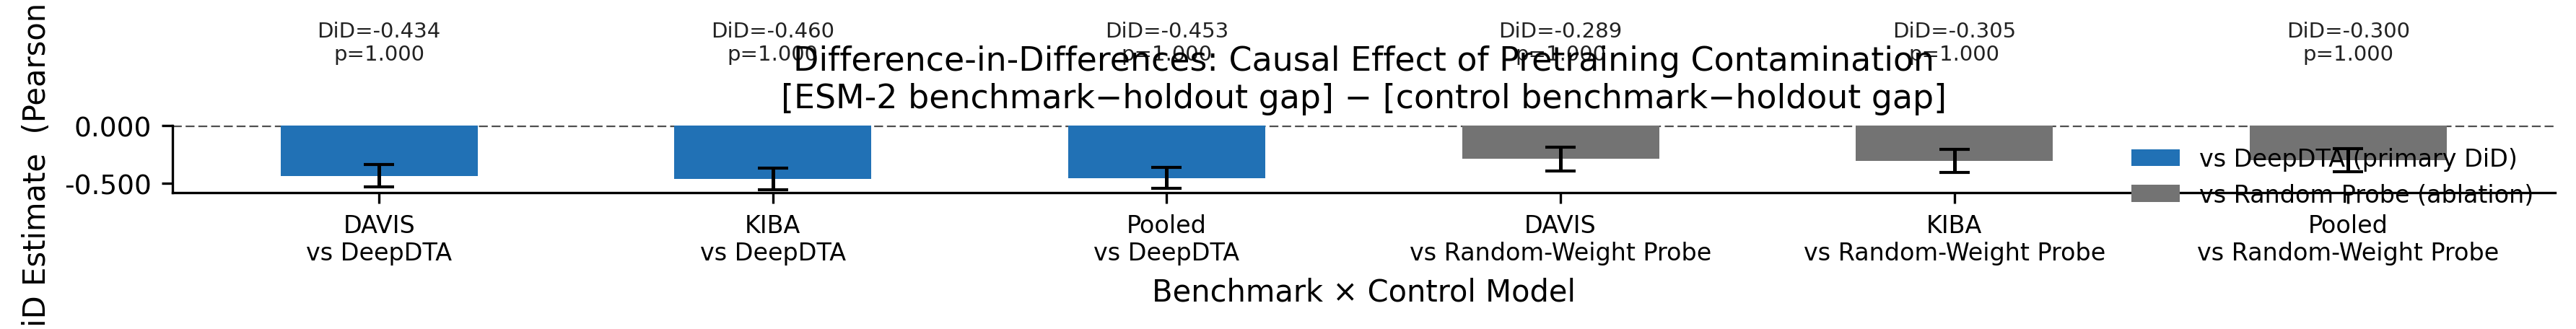
\includegraphics[width=0.85\linewidth]{figures/did_estimates.png}
\caption{DiD estimates with 95\% bootstrap CIs. Blue bars: primary DiD (ESM-2 vs.\
DeepDTA). Grey bars: ablation DiD (ESM-2 vs.\ random-weight probe). The dashed line at
zero marks the boundary of the contamination hypothesis; all estimates are significantly
below it.}
\label{fig:did}
\end{figure}

\subsection{Contaminated vs.\ Clean Subset Comparison}

Table~\ref{tab:breakdown} reports Pearson $r$ stratified by contamination class.
Note the severe class imbalance: Davis has only 84 clean test pairs (1.4\%), limiting
statistical power for that comparison.

\begin{table}[h]
\centering
\caption{Pearson $r$ on contaminated (Tanimoto $\geq 0.6$) vs.\ clean ($< 0.6$) test subsets.
Davis clean $n=84$; KIBA clean $n=1{,}056$.}
\label{tab:breakdown}
\begin{tabular}{lcccccc}
\toprule
 & \multicolumn{3}{c}{\textbf{Davis}} & \multicolumn{3}{c}{\textbf{KIBA}} \\
\cmidrule(lr){2-4}\cmidrule(lr){5-7}
\textbf{Model} & \textbf{Contam.} & \textbf{Clean} & $\Delta$ & \textbf{Contam.} & \textbf{Clean} & $\Delta$ \\
\midrule
ESM-2 probe  & 0.667 & 0.615 & $+$0.052 & 0.788 & 0.734 & $+$0.054 \\
DeepDTA      & 0.710 & 0.631 & $+$0.079 & 0.855 & 0.823 & $+$0.032 \\
Random Probe & 0.650 & 0.655 & $-$0.005 & 0.787 & 0.779 & $+$0.008 \\
\bottomrule
\end{tabular}
\end{table}

The random probe exhibits a near-zero contaminated$-$clean gap ($\Delta \approx 0$),
consistent with no pretraining memory.
ESM-2 shows a small positive gap ($\Delta \approx 0.05$), but this is comparable to or
smaller than DeepDTA's gap---a model that cannot be contaminated by pretraining.
This pattern is consistent with the contaminated subset being intrinsically easier to predict
(more training analogues), rather than reflecting memorisation by pretrained encoders.

\begin{figure}[h]
\centering
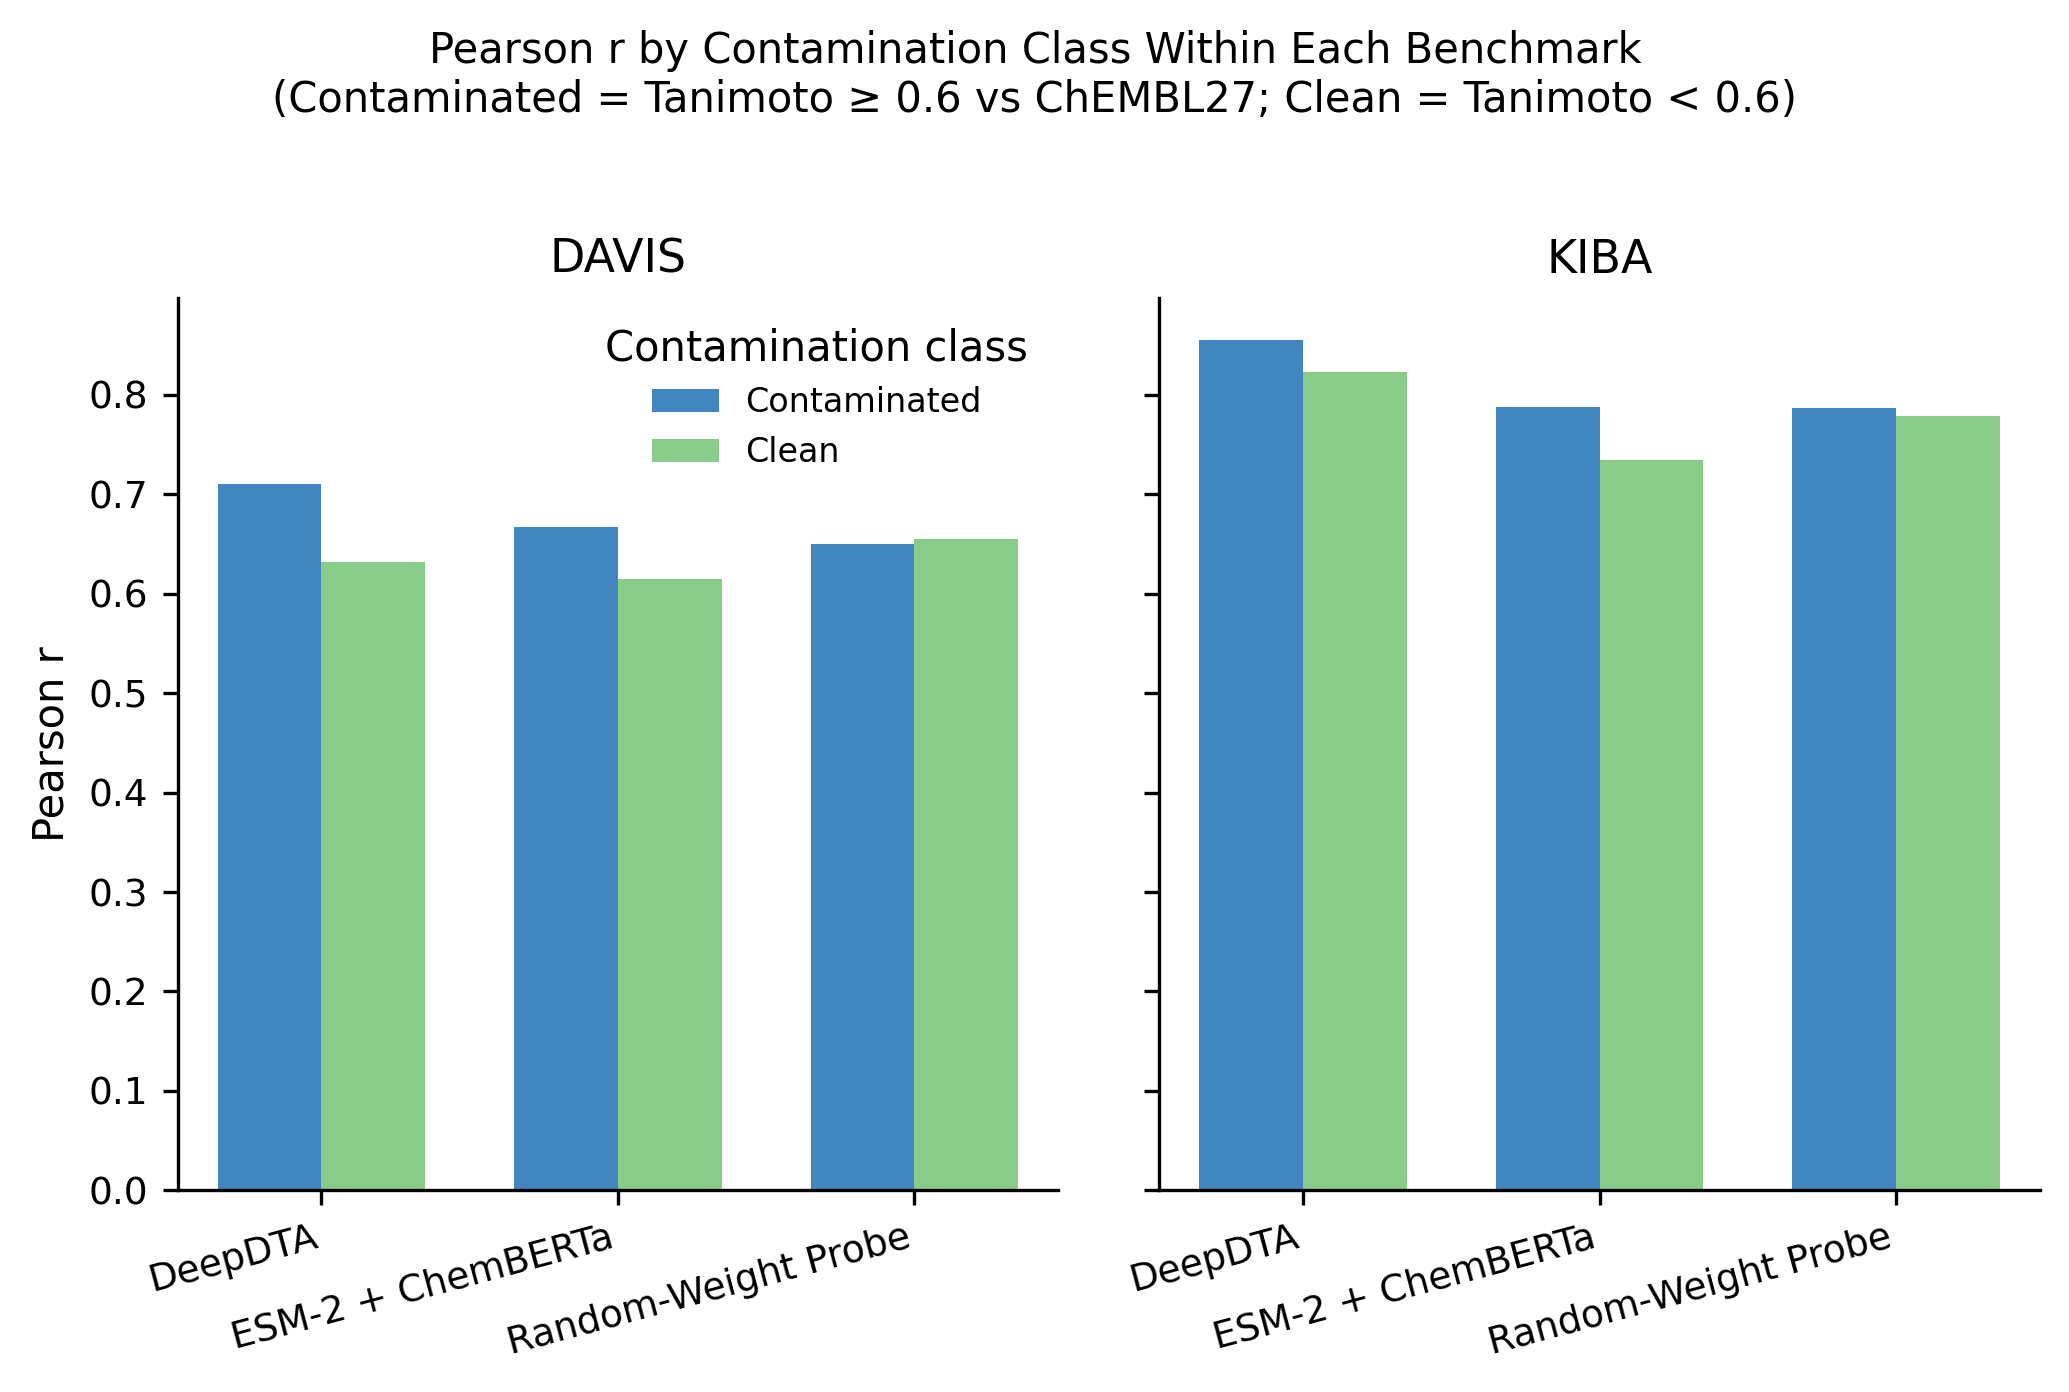
\includegraphics[width=0.85\linewidth]{figures/contamination_breakdown.png}
\caption{Pearson $r$ by contamination class (contaminated = Tanimoto $\geq 0.6$
vs.\ ChEMBL27; clean $< 0.6$) for each model and benchmark.}
\label{fig:breakdown}
\end{figure}

\subsection{Continuous Dose-Response (Tanimoto vs.\ Error)}

Figure~\ref{fig:tanimoto} and Table~\ref{tab:spearman} report Spearman $\rho$ between
compound similarity and prediction error.
Under the contamination hypothesis, we expect $\rho < 0$ (higher similarity $\to$ smaller
error).
All three models show $|\rho| < 0.02$; none are significantly negative for ESM-2 or the
random probe.
DeepDTA shows a weak negative $\rho = -0.018$ ($p = 0.002$), likely attributable to
training-set overlap: contaminated compounds have structural analogues in the training set,
making them slightly easier for any model regardless of pretraining.

\begin{table}[h]
\centering
\caption{Spearman $\rho$ between max Tanimoto similarity to ChEMBL27 and $|\hat{y} - y|$.
Negative $\rho$ would support the contamination hypothesis.}
\label{tab:spearman}
\begin{tabular}{lccc}
\toprule
\textbf{Model} & $\boldsymbol{\rho}$ & $\boldsymbol{p}$ & $\boldsymbol{n}$ \\
\midrule
ESM-2 + ChemBERTa & $+$0.009 & 0.133 & 29,663 \\
DeepDTA           & $-$0.018 & 0.002 & 29,663 \\
Random Probe      & $-$0.006 & 0.269 & 29,663 \\
\bottomrule
\end{tabular}
\end{table}

\begin{figure}[h]
\centering
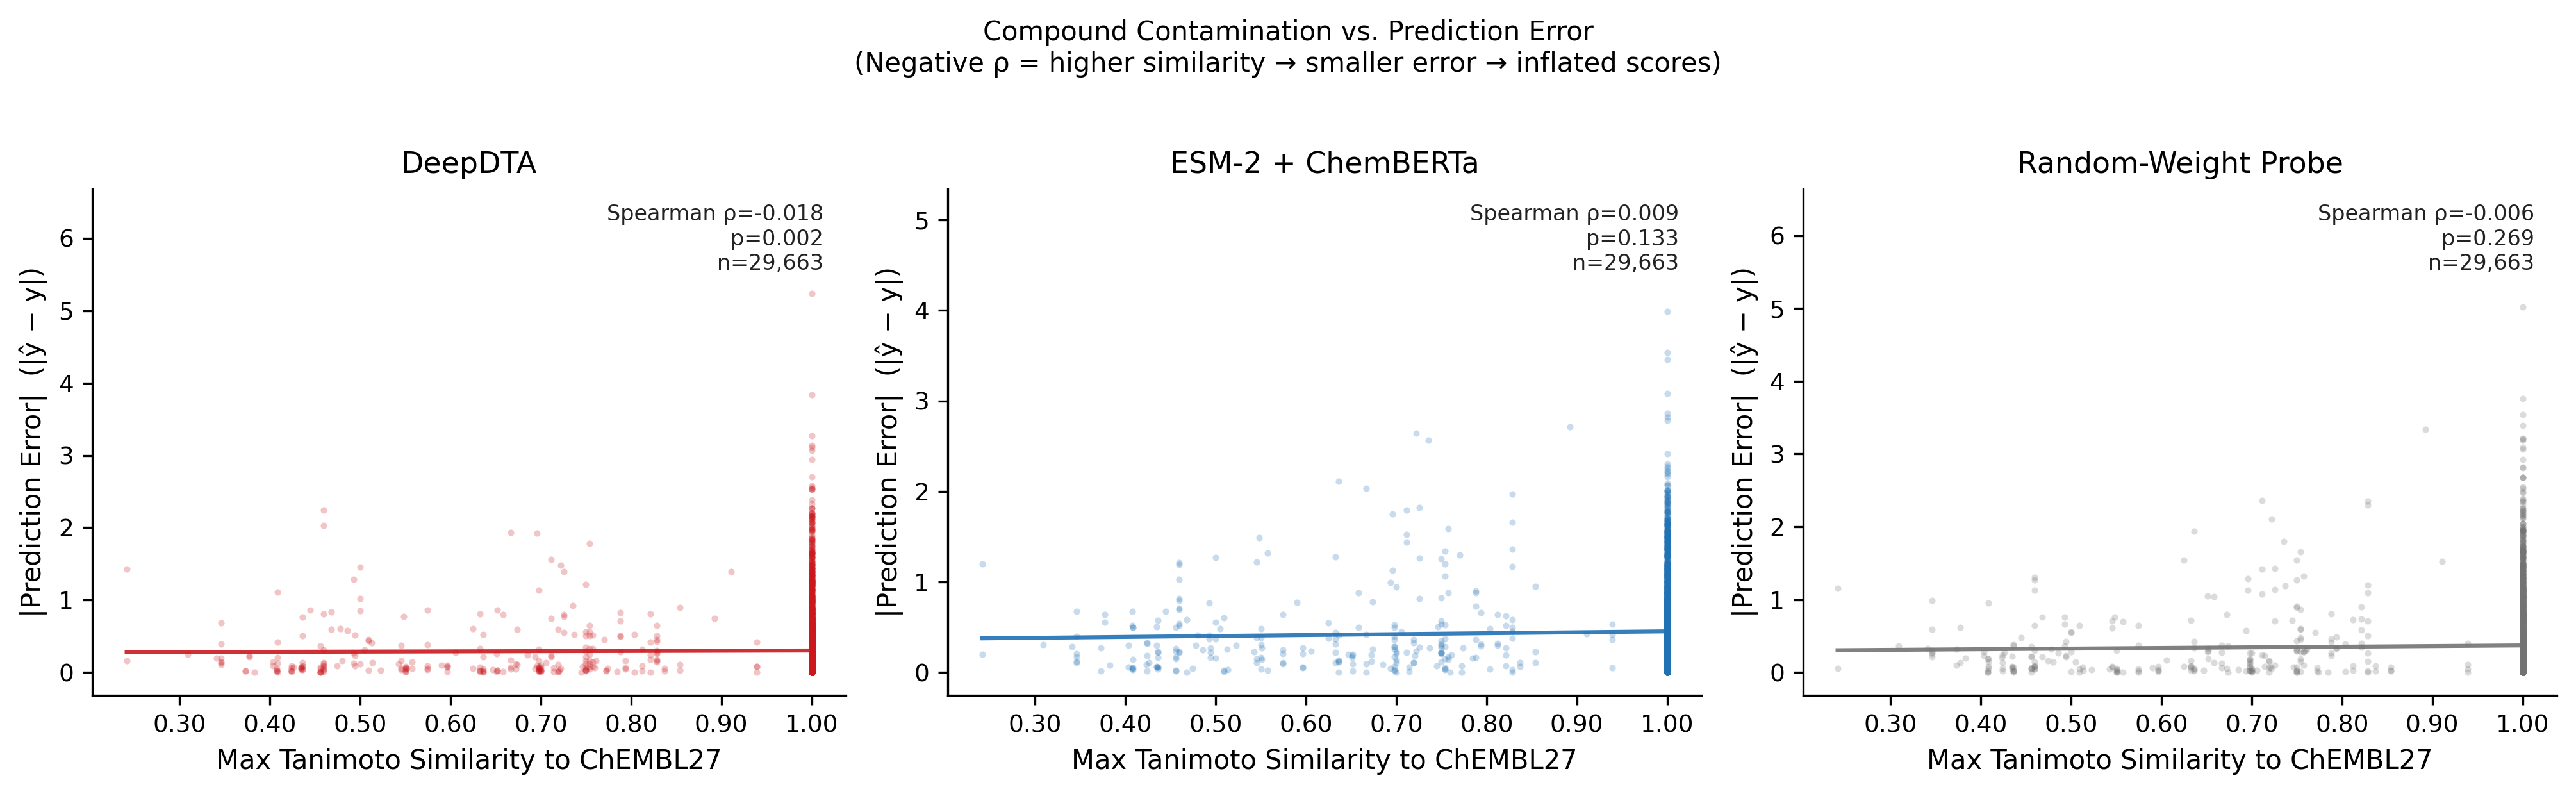
\includegraphics[width=0.95\linewidth]{figures/tanimoto_error_scatter.png}
\caption{Compound Tanimoto similarity to ChEMBL27 vs.\ absolute prediction error, with
linear trend and Spearman $\rho$. Near-flat trends across all models are inconsistent with
the contamination hypothesis.}
\label{fig:tanimoto}
\end{figure}

\begin{table}[h]
\centering
\caption{Contamination class balance in the test sets.}
\label{tab:balance}
\begin{tabular}{lrrrr}
\toprule
\textbf{Dataset} & \textbf{Total $n$} & \textbf{Contaminated} & \textbf{Clean} & \textbf{\% Contaminated} \\
\midrule
Davis & 6,012 & 5,928 & 84  & 98.6\% \\
KIBA  & 23,651 & 22,595 & 1,056 & 95.5\% \\
\bottomrule
\end{tabular}
\end{table}

\subsection{Protein Contamination}

All 607 unique proteins in the combined benchmark+holdout set achieve $\geq 90\%$ sequence
identity to a UniRef50 entry via MMseqs2.
This zero-variance result means stratification by protein contamination class is not possible
for Davis/KIBA: every benchmark protein is maximally contaminated by this definition.
We report this as an explicit null finding: Davis and KIBA consist exclusively of
well-characterised human kinases, making them structurally unsuitable for testing
protein-level pretraining contamination.

\section{Discussion}

\subsection{Interpreting the Negative DiD}

A negative DiD means ESM-2's benchmark-holdout performance gap is \emph{smaller} than
the control model's gap.
The absolute values make this concrete: ESM-2's within-model gap is 0.744 Pearson $r$ units
(benchmark 0.761, holdout 0.017); DeepDTA's gap is 1.198 units (benchmark 0.823, holdout
$-0.375$).
Far from benefiting disproportionately from the contaminated benchmark, ESM-2
\emph{generalises better} than DeepDTA to the clean holdout.
This is plausibly because ESM-2's universal protein representations, trained on all of
UniRef50, encode biologically relevant features that are not purely task-specific.
DeepDTA's 1D CNN, trained exclusively on task data, learns benchmark-specific sequence
patterns that fail to transfer.

\subsection{The Random Probe Ablation}

The near-identical benchmark performance of the random-weight probe (Davis $r = 0.650$,
KIBA $r = 0.786$) and ESM-2 (Davis $r = 0.666$, KIBA $r = 0.786$) is the most striking
finding in this study.
Random Gaussian projections of the correct dimensionality, combined with a well-regularised
MLP, match pretrained encoders on both benchmarks.
This implies that benchmark performance is dominated by the MLP's capacity to fit the data
distribution, not by the quality of molecular or protein representations.
The benchmark structure---kinase activity data with limited structural diversity---may
provide sufficient implicit regularisation that the MLP converges to similar solutions
regardless of input representation quality.

\subsection{The Generalisation Gap}

All three models produce near-zero or negative Pearson $r$ on the holdout.
This is not a statistical artefact: the holdout contains 801 real binding measurements
from ChEMBL34, with the same quality controls as the benchmarks.
The structural novelty gate (Tanimoto $< 0.4$) ensures the holdout tests extrapolation,
not interpolation.
The ESM-2 probe ($r = 0.017$, 95\% CI $[-0.051, 0.086]$) is not statistically different
from random.

This result reframes the question for the field.
Contamination is not inflating Davis/KIBA scores---but the scores do not measure what matters.
A model that achieves $r = 0.786$ on KIBA and $r = 0.017$ on structurally novel compounds
provides little assurance of real-world utility.

\subsection{Limitations}

\paragraph{Corpus proxy.}
ChemBERTa-zinc-base-v1 was pretrained on a ZINC subset ($\sim$100K molecules), not ChEMBL27.
The correct contamination reference for ChemBERTa is ZINC, but the specific training split is
not publicly available, and the full ZINC database ($>250$M compounds) is impractical for
FPSim2 similarity search.
We use ChEMBL27 as a conservative proxy; since ZINC and ChEMBL overlap substantially,
this is likely to capture most contaminated compounds.

\paragraph{Davis clean subset.}
With only 84 clean test compounds in Davis (1.4\% of the test set), the contaminated
vs.\ clean comparison for Davis lacks statistical power.
The near-universal contamination of Davis reflects its age and limited chemical diversity.

\paragraph{Protein contamination.}
Davis and KIBA consist exclusively of human kinases, all of which are identical to UniRef50
entries.
Testing protein-level contamination requires benchmarks with structurally diverse targets
spanning a wider taxonomic range.

\paragraph{Parallel trends.}
The DiD relies on the parallel trends assumption: that the control model's benchmark-holdout
gap reflects difficulty alone, not contamination.
DeepDTA's catastrophic holdout failure ($r = -0.375$) could in principle reflect
benchmark-specific overfitting that is not present in ESM-2, violating this assumption.
We note that the random-probe control---which cannot overfit to benchmark representations
the same way---yields a consistent negative DiD ($-0.300$), supporting our interpretation.

\section{Conclusion}

We conducted a causal difference-in-differences analysis of pretraining contamination in
drug-target interaction benchmarks.
Using Davis and KIBA as contaminated arms and a clean ChEMBL34 holdout as the uncontaminated
arm, we find:

\begin{enumerate}
  \item \textbf{No contamination inflation.}
    The DiD estimate is negative across all benchmarks and control models ($p = 1.0$
    against the contamination hypothesis), with or without a random-weight ablation as control.
  \item \textbf{Pretraining provides negligible benchmark signal.}
    A random-weight probe nearly matches ESM-2+ChemBERTa on Davis and KIBA.
    Benchmark performance is driven by data structure and MLP capacity, not representation quality.
  \item \textbf{All models fail on novel chemistry.}
    Every model---pretrained, from-scratch, and random---achieves near-chance performance
    on the clean holdout.
    Davis and KIBA do not measure generalisation.
  \item \textbf{Protein contamination is untestable on these benchmarks.}
    Every Davis/KIBA target is maximally similar to UniRef50 (human kinases);
    no stratification is possible.
\end{enumerate}

The actionable recommendation for the field is not to chase contamination-corrected
Davis/KIBA scores, but to retire these benchmarks as primary evaluations in favour of
prospective tests on structurally novel compounds or targets outside the kinome.

\section*{Reproducibility}

All code, data splits, and result files are available at:
\begin{center}
\url{https://github.com/swmeyer1979/dti-contamination}
\end{center}
The pipeline is fully automated and can be re-run with \texttt{bash run\_pipeline\_revised.sh}.
Pretrained encoder weights are downloaded automatically from HuggingFace.
Data splits and contamination labels are included in the repository.
The clean holdout is derived from ChEMBL34, which requires a ChEMBL account for bulk access;
we include the processed holdout parquet directly.

\section*{Acknowledgements}

No external funding. Analysis performed on a MacBook Pro (M-series, MPS acceleration).

\bibliographystyle{abbrvnat}
\bibliography{references}

\end{document}
